\chapter{Kết luận và hướng phát triển}\label{ch:4}
\section{Kết quả đạt được}\label{sec:4.1}
\subsection{Xét các hàm 1 chiều}\label{subsec:3.2.1}
\begin{itemize}
    \item Xét hàm f(x) có 3 đỉnh nhọn lấy tích phân trên miền xác định [0,1]
    \begin{align}
        I = \int_{0}^{1}\left(\frac{1}{(x-0.25)^2 +10^-6} +\frac{1}{(x-0.5)^2 +10^-6}+\frac{1}{(x-0.75)^2 +10^-6}\right)dx
    \end{align}
    \begin{figure}[H]
        \centering
        \includegraphics[width=0.5\textwidth]{1d_x02505075.png}
        \caption{Dạng đồ thị của f(x)}\label{hinh3.2}
    \end{figure}
    \begin{table}[H]
        \centering
        \begin{tabular}{ |c|c|c|c|c| }
         \hline
         \multicolumn{1}{|c}{Số mẫu} & \multicolumn{1}{|c|}{Số vòng lặp} & \multicolumn{1}{|c|}{Kết quả I} & \multicolumn{1}{|c|}{Sai số $\sigma$} & \multicolumn{1}{|c|}{Kết quả giải tích số} \\
         \hline
         10000 & 1  & 9370.37 & 29.30 & 9410.11 \\
         \hline
         10000 & 10  & 9410.12 & 0.07 & 9410.11 \\
         \hline
         10000 & 100  & 9410.12 & 0.02 & 9410.11 \\
         \hline
        \end{tabular}
        \caption{Bảng kết quả tích phân 1 chiều}
        \label{1d_x02505075}
       \end{table}
    
    %===========================
     %===========================
    \item Xét hàm f(x) có đỉnh nhọn cao và hẹp, lấy tích phân trên miền xác định $[10^{-10},2]$
    \begin{align}
        I = \int_{10^{-10}}^{1}\left({\frac{1}{x}+20exp(-10^{-4}(x-1)^2)}\right)
    \end{align}
    \begin{figure}[H]
        \centering
        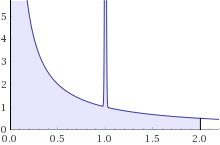
\includegraphics[width=0.5\textwidth]{1d_20.png}
        \caption{Dạng đồ thị của f(x)}\label{hinh3.2}
    \end{figure}
    \begin{table}[H]
        \centering
        \begin{tabular}{ |c|c|c|c|c| }
         \hline
         \multicolumn{1}{|c}{Số mẫu} & \multicolumn{1}{|c|}{Số vòng lặp} & \multicolumn{1}{|c|}{Kết quả I} & \multicolumn{1}{|c|}{Sai số $\sigma$} & \multicolumn{1}{|c|}{Kết quả giải tích số} \\
         \hline
         10000 & 1  & 11.4698 & 0.6 & $log(2.10^2) + 2.sqrt(\frac{\pi}{10})$ \\
         \hline
         10000 & 10  & 24.0734 & 0.0002 & $log(2.10^2) + 2.sqrt(\frac{\pi}{10})$ \\
         \hline
         10000 & 100  & 24.0734 & 4.039e-05 & $log(2.10^2) + 2.sqrt(\frac{\pi}{10})$ \\
         \hline
        \end{tabular}
        \caption{Bảng kết quả tích phân 1 chiều}
        \label{1d_x02505075}
       \end{table}
    

\end{itemize}

\subsection{Xét các hàm 2 chiều}\label{subsec:3.2.2}
\begin{itemize}
    \item Xét tích phân 
    \begin{align}
        I=\int_{-1}^{1}\int_{-1}^{1} {exp(-20(x^2+y^2))}dxdy
    \end{align}
    
    \begin{table}[H]
        \centering
        \begin{tabular}{ |c|c|c|c|c| }
         \hline
         \multicolumn{1}{|c}{Số mẫu} & \multicolumn{1}{|c|}{Số vòng lặp} & \multicolumn{1}{|c|}{Kết quả I} & \multicolumn{1}{|c|}{Sai số $\sigma$} & \multicolumn{1}{|c|}{Kết quả giải tích số} \\
         \hline
         10000 & 1  & 0.157403  & 0.0003 & $\approx 0.15708$ \\
         \hline
         10000 & 10  &  0.157029 & 0.0002 & $\approx 0.15708$ \\
         \hline
         10000 & 100  & 0.156698 & 0.0001 & $\approx 0.15708$ \\
         \hline
        \end{tabular}
        \caption{Bảng kết quả tích phân 2 chiều}
        \label{2d_xy}
       \end{table}
    
    

\end{itemize}

\subsection{Xét các hàm 3 chiều}\label{subsec:3.2.3}
\begin{itemize}
    \item Xét tích phân sau 
    \begin{align}
        I=\int_{0}^{1}\int_{0}^{1} \int_{0}^{1} {\frac{1}{xyz+10^{-6}}}dxdydt
    \end{align}
    \begin{table}[H]
        \centering
        \begin{tabular}{ |c|c|c|c|c| }
         \hline
         \multicolumn{1}{|c}{Số mẫu} & \multicolumn{1}{|c|}{Số vòng lặp} & \multicolumn{1}{|c|}{Kết quả I} & \multicolumn{1}{|c|}{Sai số $\sigma$} & \multicolumn{1}{|c|}{Kết quả giải tích số} \\
         \hline
         10000 & 1  & 574.415  & 125.527 & 462.216 \\
         \hline
         10000 & 10  & 461.803  & 0.425806 & 462.216 \\
         \hline
         10000 & 100  & 462.31 & 0.0964302 & 462.216 \\
         \hline
        \end{tabular}
        \caption{Bảng kết quả tích phân 3 chiều}
        \label{3d_xyz}
       \end{table}
\end{itemize}

\subsection{Xét các hàm 4 chiều}\label{subsec:3.2.4}
\begin{itemize}
    \item Xét hàm f(x) có 3 đỉnh nhọn lấy tích phân trên miền xác định [0,1]
    \begin{align}
        I^n=\left(\frac{1}{a{\pi}^{\frac{1}{2}}}\right)^n\int_{0}^{1} 
        {d^nx\exp\left({-\sum_{i=1}^n{\frac{(x_i-0.5)^2}{a^2}}}\right)}
    \end{align}
    Với $n=4, a=0.1$
    \begin{table}[H]
        \centering
        \begin{tabular}{ |c|c|c|c|c| }
         \hline
         \multicolumn{1}{|c}{Số mẫu} & \multicolumn{1}{|c|}{Số vòng lặp} & \multicolumn{1}{|c|}{Kết quả I} & \multicolumn{1}{|c|}{Sai số $\sigma$} & \multicolumn{1}{|c|}{Kết quả giải tích số} \\
         \hline
         10000 & 1  &  1.18126 & 0.1271 & 1 \\
         \hline
         10000 & 10  & 1.00069 & 0.00126 & 1 \\
         \hline
         10000 & 100  & 0.999867 & 0.0004 & 1 \\
         \hline
        \end{tabular}
        \caption{Bảng kết quả tích phân 4 chiều}
        \label{4d_xyzt}
       \end{table}
\end{itemize}

\section{Kết luận}\label{sec:4.2}
Đề tài tập trung giải quyết các bài toán tích phân trong không gian 1 chiều đến 4 chiều.
Kết quả ước tính tích phân từ báo cáo khóa luận so với kết quả chính xác từ phương pháp giải tích số gần như bằng nhau.
Sự chênh lệch của ước tính tích phân thì nằm trong khoảng sai số mà phương pháp tính toán được. 
Vì thế, ước tính tích phân được xem như là chính xác so với kết quả thực tế. 
Ngoài ra sản phẩm của đề tài đã xử lý thành công các bài toán có hàm lấy tích phân có các đỉnh nhọn cao và hẹp trong không gian đa chiều (1 chiều đến 4 chiều).\par
Bên cạnh việc xử lý được các vấn đề đã đề cập ở trên thì báo cáo khóa luận vẫn chưa xử lý chính xác các bài toán lớn hơn 4 chiều. 
Và đôi khi vẫn cho ra ước tính sai lệch khá lớn so với kết quả chính xác đối với các hàm tích phân đặc biệt trong không gian 4 chiều.  
\section{Hướng phát triển đề tài}\label{sec:4.1}
Dựa vào kết quả và phân tích đạt được thì đề tài cần phát triển thêm khả năng tính toán các tích phân lớn hơn 4 chiều. 
Tìm hiểu và phân tích các kết quả từ các thuật toán tính tích phân khác của nhiều tác giả khác nhau, để từ đó có thể tối ưu hóa ước tính tích phân.